\documentclass[titlepage]{article}
\usepackage[pdftex]{graphicx}

% Title
\title{Lab 1: Simple Harmonic Motion}
\author{Yacin Nadji}
\date{September 15th, 2006}

\begin{document}
\maketitle

\section{Statement of Objective}\label{sec:obj}
The purpose of this lab was to study the effects of Simple Harmonic Motion through the use of springs and pendulums, and to familiarize ourselves with the oscilloscope.

\section{Theory}\label{sec:theory}
When an object exhibits periodic motion (something that can be attributed to a trig function of some sort), the object is said to be in \textbf{harmonic motion}. The most easily understood and fundamental type of this is known as Simple Harmonic Motion (SHM).\\
\\
A string that is stretched past its point of equilibrium and allowed to contract freely will exhibit SHM. If observed, it's very easy to see a spring in such motion is periodic, and excluding all external forces, it would continue to move this way perpetually.\\
\\
A pendulum will operate in the same fashion. When pulled to one side and allowed to fall, the pendulum will oscillate between it's point of equilibrium, showing a constant gain/loss of potential/kinetic energy. If done in a vacuum, it would continue like this forever.

\section{Equipment List}\label{sec:equipment_list}
\begin{itemize}
\item[*] Ring Stand
\item[*] Spring
\item[*] Masses
\item[*] Timer
\item[*] Function Generator
\item[*] DC Power Source
\item[*] Oscilloscope
\end{itemize}

\section{Procedure}\label{sec:procedure}
\subsection{Part A}\label{sub:part_a}
We attached the spring to a ring stand and hung a mass from the end of the spring. Holding the mass at the springs equilibrium point, we let it drop and the spring was allowed to oscillate. The time for 10 oscillations was recorded. This was repeated several times to get an average time, and was repeated five times for different masses.

\subsection{Part B}\label{sub:part_b}
We attached a string to the ring stand and hung a mass from the other end. The mass was displaced to one side and allowed to swing freely. Once again, we recorded the time for 10 oscillations. This was repeated several times to get an average time, and was repeated five times with different lengths of string.

\subsection{Part C}\label{sub:part_c}
We set the generator to a specific frequency of known value, and measurements were taken. This was done multiple times, and the measurements were then used to compare the given frequency to the frequency read by the oscilloscope.

\section{Data}\label{sec:data}
\subsection{Part A}\label{sub:part_a}

Spring Oscillations
\begin{tabular}{cccccc}
\hline
Mass (g) & 10 & 20 & 30 & 40 & 50\\
\hline
Time (sec) & 3.60 & 4.58 & 5.62 & 6.15 & 7.04\\
\hline
$T$ & 0.360 & 0.458 & 0.562 & 0.615 & 0.704\\
\hline
$T^2$ & 0.129 & 0.209 & 0.315 & 0.378 & 0.495\\
\hline
\end{tabular}

\subsection{Part B}\label{sub:part_b}

Pendulum Oscillations
\begin{tabular}{cccccc}
\hline
Length (m) & .10 & .20 & .30 & .40 & .50\\
\hline
Time (s) & 6.81 & 9.33 & 11.05 & 11.98 & 13.98\\
\hline
$T$ & 0.681 & 0.933 & 1.105 & 1.198 & 1.398\\
\hline
$T^2$ & 0.463 & 0.870 & 1.220 & 1.435 & 1.954\\
\hline
\end{tabular}


\section{Analysis of Data}\label{sec:analysis_of_data}

\subsection{Part A}\label{sub:part_a}
The equation we used to relate the mass and the spring to the time it takes to complete an oscillation is
\begin{equation}
	T = 2 \pi \sqrt{\frac{m}{k}}
\end{equation}
By squaring both sides of the equation, we get
\begin{equation}
	T^2 = \frac{4 \pi^2}{k} m
\end{equation}
When the time is squared, and the mass attached to the spring are plotted in a linear fashion, the slope of the line is equal to $\frac{4 \pi^2}{k}$. The value of $k$ can then be found by using the equation
\begin{equation}
	k = -\frac{mg}{x}
\end{equation}
\\
\\
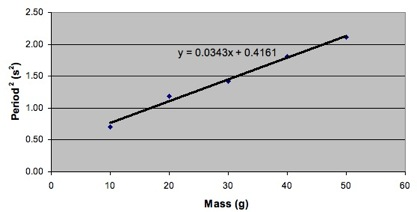
\includegraphics{graphA.jpg}
\\
Using the approximate slope we have calculated, we can derive the constant $k$.

\[
	0.0343 = \frac{4 \pi^2}{k}
\]
\[
	k = 1150.97
\]
The percent error can now be tabulated
\[
	\% Error = \frac{|1264.52 - 1150.97|}{1264.52} * 100 = 8.98\%
\]

\subsection{Part B}\label{sub:part_b}
The three main factors of this experiment, the gravitational acceleration, the period of the oscillation and the length of the string of the pendulum are all related through the equation
\begin{equation}
	T = 2 \pi \frac{L}{g}
\end{equation}
We can do some minor manipulation to the equation and get a more useful one
\begin{equation}
	T^2 = \frac{4 \pi^2}{g} L
\end{equation}
When this function is plotted, it yields a linear regression, with the slope of the line being represented by $\frac{4 \pi^2}{g}$.
\\
\\
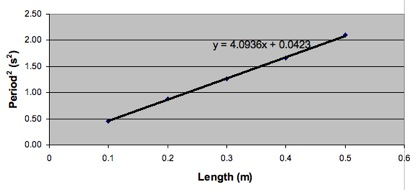
\includegraphics{graphB.jpg}
\\
Now that we have an approximate regression line, we can use this to determine the value of $g$

\[
	4.0936 = \frac{4 \pi^2}{g}
\]
\[
	g = 9.644 \frac{m}{s^2}
\]

Now, we determine the percent error
\[
	\% Error = \frac{|9.81 - 9.64|}{9.81} * 100 = 1.69\%
\]

\subsection{Part C}\label{sub:part_c}

In order to get the oscilloscope working properly, it was necessary for us to first, zero out the oscilloscope. Similarly to zeroing out a scale or any other measuring device, this allowed us to read accurate results.\\
\\
Next, we set the DC power supply to 5 volts and the oscilloscope showed us a flat line. This makes sense, considering the amount of voltage was a constant value over time. By increasing and decreasing the value of the voltage, the line would translate itself up or down, respectively. By altering the VOLT/DIV knob, the location of the line changed as well. This changes the scale of the grid lines.\\
\\
By changing the oscilloscope channel, we were able to view the AC waveform, rather than the DC waveform. By altering the SEC/DIV knob, we changed the time scale so that only a few cycles of the waveform could be seen. We measured the time it took the wave to make one complete cycle, and by taking the inverse, we are left with the frequency. We determined this to be 1429 Hz. After this, we changed the vertical position of the wave so that it would line up with the grid lines. By counting the grid lines from the peak of the wave to 0, we could determine our amplitude.\\
\\
The function generator was set to 1500 Hz, and we calculated the value of 1429 Hz. Based on that, here's the percent error
\[
	\% Error = \frac{|1500 - 1429|}{1500} * 100 = 4.7\%
\]

\section{Discussion of Results}\label{sec:discussion_of_results}
\subsection{Part A}\label{sub:part_a}
We determined the calculated spring constant to be $k = 1264.52$. The \% Error of $8.98\%$ is pretty decent. I attribute the error mainly to the fact that we were timing the oscillations by eye, rather than using something more accurate, like a photo gate. Because of this variation, it's understandable to have a slight discrepancy between the true value.

\subsection{Part B}\label{sub:part_b}
We calculated the value of $g$ to be $9.64 \frac{m}{s^2}$. Our \% Error of $1.69\%$ is phenomenal in my mind, considering the number of outside forces that could easily alter our data. Once again, I think the largest amount of the error is coming from the fact that we judged the oscillations by eye, and had to manually determine the time, rather than using photo gates. Had we used photo gates, I'm sure the results would've been even better.

\subsection{Part C}\label{sub:part_c}
The measured amplitudes for both the DC and AC sources were very accurate and consistent. The calculated frequency for the wave was 1429 Hz, despite the fact that the function generator was set to 1500 Hz. This 4.7\% error was most likely due to error on our part, as reading the exact measurement off the oscilloscope is relatively difficult.

\section{Conclusions}\label{sec:conclusions}
The relatively accurate and consistent results provided by our data reinforces the validity of the equations presented to us in class. You can see this by looking at the tables for Part A and B. It is very clear that the linear regression is quite accurate based on our data, and the linear regression calculates the constants $k$ and $g$ accurately. The cause for error is obviously on our part, considering we could've used for more accurate methods of timing than the human eye and hand.

\end{document}